\chapter{Model description}
The aim of the model described in this paper is to succesfully model the vertical distribution of one phytoplankton species in an open ocean setting. The model is relatively simple, and to some extent is built upon the models mentioned in \cite{RYABOV2010120}, \cite{HUISMAN2002} and \cite{BECKMANN2007}. The model is modelling phytoplankton based on a bottom-up control, meaning that control of phytoplankton from grazing and higher trophic levels have been disregarded. The bottom-up control is in this instance reflected in the two possible limiting factors: nutrients or light intensity. It could be expanded to include detritus as another state variable, but that has not yet been implemented. It is built up as an advection-reaction-diffusion model, and is to some extent built upon the model mentioned in \cite{RYABOV2010120}. A model illustration can be seen in \cref{fig:ModelIllustration}. 

\begin{figure}[H]
\centering
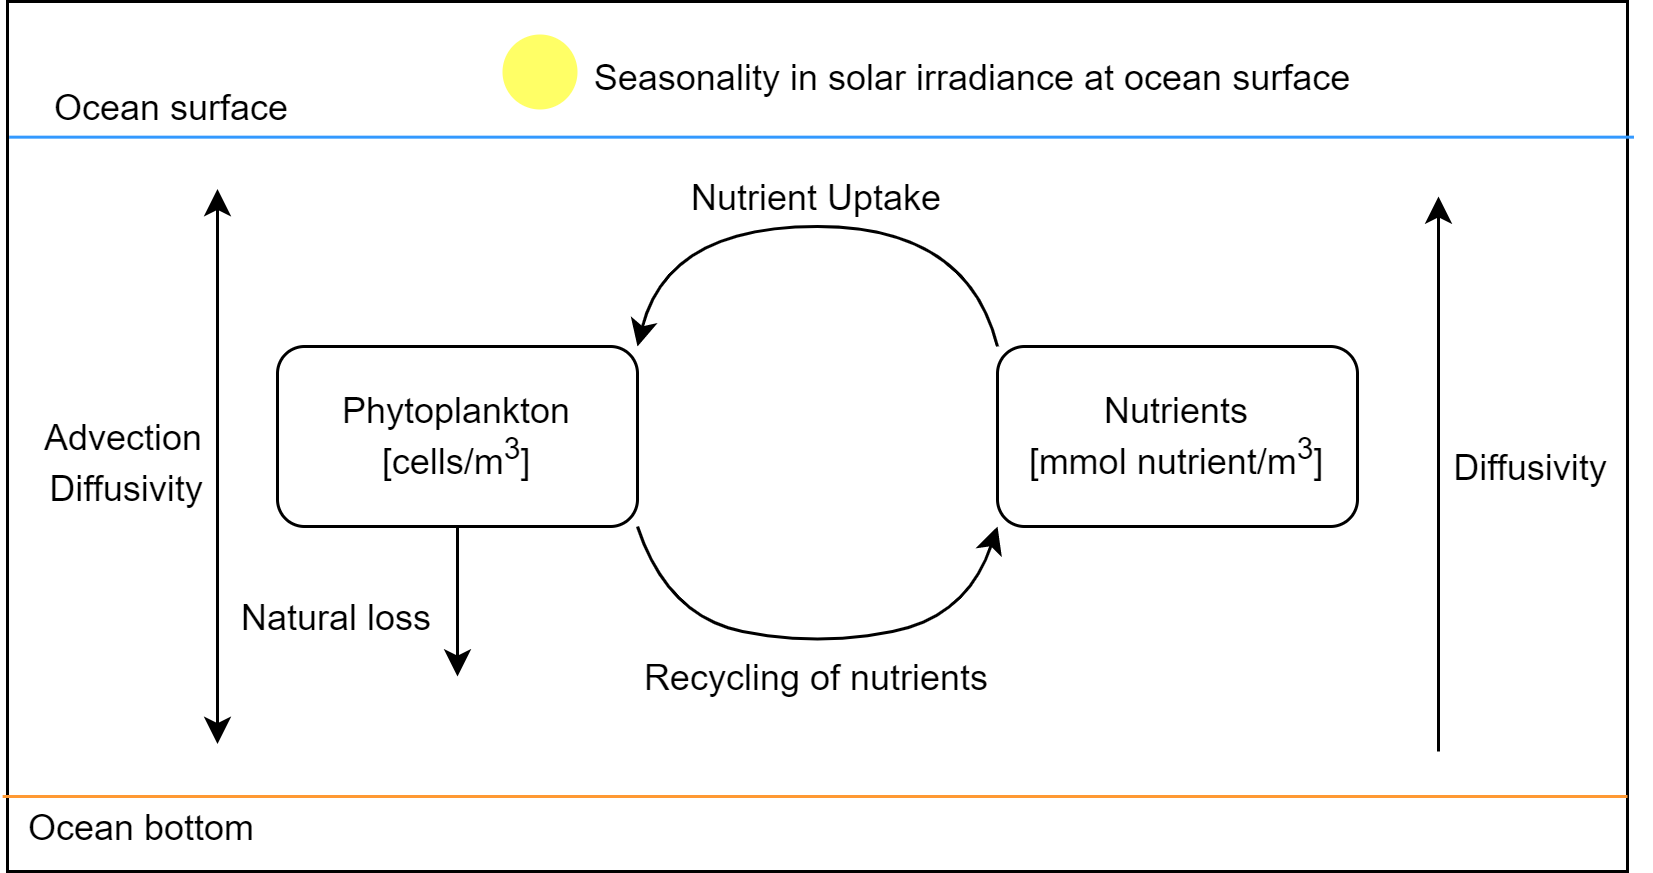
\includegraphics[width=.7\linewidth]{Pictures/ModelIllustration.png}
\caption{A graphical illustration of the model and its state variables.}
\label{fig:ModelIllustration}
\end{figure}

\section{Description of equations} \label{DescripEq}
The model consists of three state variables that is phytoplankton concentration \textit{P} at time \textit{t} and depth \textit{z}, denoted as \textit{P(z,t)}, and nutrient concentration denoted as \textit{N(z,t)} and light intensity \textit{I(z,t)}. 
The system dynamics between nutrients and phytoplankton is modelled by the following equations:
\begin{equation} \label{eq:Peq}
    \frac{\partial P}{\partial t} = \textcolor{green}{growth} - \textcolor{red}{loss} - \textcolor{yellow}{sinking} + \textcolor{blue}{mixing} = \textcolor{green}{\mu P} - \textcolor{red}{lP} - \textcolor{yellow}{u\frac{\partial P}{\partial z}} + \textcolor{blue}{D\frac{\partial P}{\partial z}}
\end{equation}

\begin{equation} \label{eq:Neq}
    \frac{\partial N}{\partial t} = - \textcolor{green}{uptake} + \textcolor{red}{recycling} + \textcolor{blue}{mixing} = - \textcolor{green}{\alpha \mu P} + \textcolor{red}{\varepsilon \alpha lP} + \textcolor{blue}{D\frac{\partial N}{\partial z}}
\end{equation}

Here $\mu(N,I)$ is the growth rate for phytoplankton, $l$ is the mortality of phytoplankton, $u$ is the velocity of the downwards advection, $D$ is the diffusion by mixing, $\alpha$ is the nutrient concentration of a phytoplankton cell and $\varepsilon$ is the recycling coefficient of phytoplankton.
As seen in \cref{eq:Peq} and \cref{eq:Neq}, the equations are coupled by the growth rate of phytoplankton, $\mu(N,I)$. The growth rate is dependent on available nutrients and light intensities. In order to model growth being either nutrient or light limited, von Liebig's law of minimum has been applied in the following way:
\begin{equation} \label{eq:Growtheq}
    \mu(N,I) = \mu_{max} \: min\left( \frac{N}{H_N + N},\frac{I}{H_I + I}\right)
\end{equation}
Here $\mu_{max}$ is the maximum growth rate for phytoplankton, $H_N$ is the half-saturation constant for nutrients and $H_I$ is the half-saturation constant for light.
The light is assumed to dissipate exponentially with depth according to Lambert-Beer's law:
\begin{equation} \label{eq:Ieq}
    I(z,t) = I_{surface} \: \exp\left(- k_wz - k_P \int_{0}^{z} P(\zeta, t)d\zeta \right)
\end{equation}
where $I_{surface}(t)$ is the incident light reaching the ocean surface, $k_w$ is the turbidity of the water and $k_P$ is the light absorption coefficient of phytoplankton. The incident light reaching the ocean surface is assumed to vary seasonally:
\begin{equation} \label{eq:Isurfeq}
    I_{surface}(t) = I_0 - I_{amplitude}\sin{\left(\frac{\pi \phi}{180}\right)}\cos{\left(2\pi\left(\frac{t}{365}\right)\right)}
\end{equation}
where $I_0$ is the assumed average incident light intensity, $I_{amplitude}$ is the amplitude coefficient for seasonal variation, $\phi$ is the latitude (fixed at 55$^\circ$N for the purpose of this paper).
For the sake of simplicity, while doing sensitivity analysis of the model, the seasonal variations in surface light intensities were disregarded and the equation for $I(z,t)$ were thus:
\begin{equation} \label{eq:Ieq2}
    I(z,t) = I_0 \: \exp\left(- k_wz - k_P \int_{0}^{z} P(\zeta, t)d\zeta \right)
\end{equation}
In this instance the incoming light intensity is fixed at the assumed annual average incident light.

The parameters used in the model equations can be found in appendix table \ref{tab:Params}.

\section{Grid properties and boundary conditions} \label{GridDescrip}
The model is utilizing a spatial grid, and the concentrations of the dependent variables are all calculated at certain spatial positions, denoted $C$, which is defined as the centre of each grid. For this paper a total depth of 300 meters and a total of 100 grids were chosen, meaning that each cell has a length of three meters, denoted $dz$. For each grid there is a flux going in ($J_{i}$) and a flux going out ($J_i+1$). In an advection-diffusion model, the fluxes can consist of both diffusive and advective, or just one of either and in this paper we assume that for phytoplankton there is both types of movements present, whereas for nutrients it is assumed that only diffusive flux is present.
\begin{figure}[h]
\centering
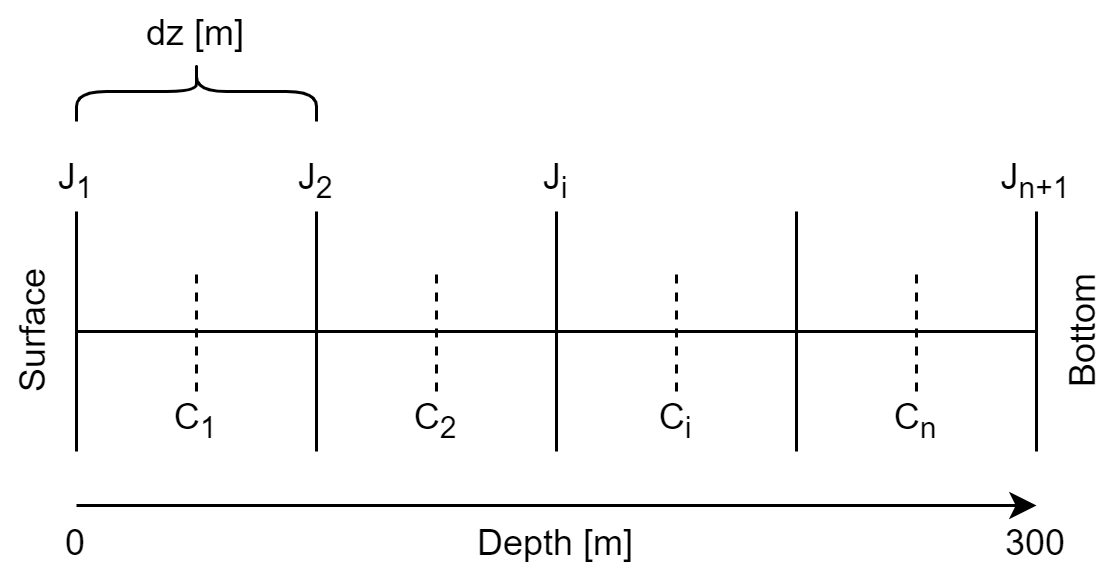
\includegraphics[width=.8\linewidth]{Pictures/GridProperties.png}
\caption{An illustration of the spatial grid utilized in the model.}
\label{fig:GridProp}
\end{figure}

The advective fluxes are calculated using the "upwind" method, where the concentration in the cell "above" is used to calculate the concentration.
\begin{equation} \label{eq:Jaeq}
    J_{a.i} \approx uC_{i-1}
\end{equation}
where $J_{a.i}$ is the advective flux flowing into cell $i$, $u$ is the velocity of the flux and $C_{i-1}$ is the concentration in the cell upstream.
The diffusive fluxes are calculated by the principle of "central differences", where a diffusive flux is only present when a gradient is present.
\begin{equation} \label{eq:Jdeq}
    J_{d.i} \approx -D\frac{C_i-C_{i-1}}{dz}
\end{equation}
where $J_{d.i}$ is the diffusive flux in the opposite direction of the gradient, $D$ is the velocity of the diffusive flux. This paper operates with a constant diffusivity, but it is possible to implement different diffusivities at depth to reflect a larger diffusivity at the surface compared to the ocean interior. 
Regarding the boundary conditions used for this paper the following were used in the surface boundary:
\begin{equation} \label{eq:SurfBound}
    F^{P}_{1} = 0, F^{N}_{1} = 0
\end{equation}
where $F$ is the total flux ($J_{a.i}+J_{d.i}$). This means that at the surface we have a closed boundary for both nutrients and phytoplankton. Regarding the bottom boundary, this paper uses the following conditions:
\begin{equation} \label{eq:BottomBound}
    F^{P}_{n+1} = 0, F^N_{n+1} = -D\frac{N_B-N_n}{dz}
\end{equation}
where there is no sinking of phytoplankton into the bottom boundary, but there is a diffusive flux of nutrients up from the bottom. One could implement a sinking of phytoplankton into the bottom boundary to reflect the remaining amount of phytoplankton that does not get recycled into nutrients.